%% LyX 2.4.2.1 created this file.  For more info, see https://www.lyx.org/.
%% Do not edit unless you really know what you are doing.
\documentclass[fontsize=12,ngerman,DIV=15, listtotoc, pointlessnumbers]{scrreprt}
\usepackage[T1]{fontenc}
\usepackage[utf8]{inputenc}
\setcounter{secnumdepth}{3}
\setcounter{tocdepth}{3}
\usepackage{xcolor}
\usepackage{babel}
\usepackage{longtable}
\usepackage{calc}
\usepackage{url}
\usepackage{amsmath}
\usepackage{graphicx}
\usepackage[a4paper]{geometry}
\geometry{verbose,lmargin=25mm,rmargin=25mm}
\usepackage{wasysym}
\usepackage[pdfusetitle,
 bookmarks=true,bookmarksnumbered=false,bookmarksopen=false,
 breaklinks=true,pdfborder={0 0 0},pdfborderstyle={},backref=false,colorlinks=false]
 {hyperref}
\hypersetup{
 hypertexnames=false}

\makeatletter

%%%%%%%%%%%%%%%%%%%%%%%%%%%%%% LyX specific LaTeX commands.
%% Because html converters don't know tabularnewline
\providecommand{\tabularnewline}{\\}

%%%%%%%%%%%%%%%%%%%%%%%%%%%%%% User specified LaTeX commands.
%\usepackage{xurl}

\usepackage{tikz}
\usepackage{tikzpagenodes} 
%\usepackage{palatino} % Fuer Schriftart Palatino (Optional)
%\usepackage{mathpazo} % Fuer Schriftart Palatino (Optional)
\usepackage[notextcomp]{stix} % Fuer Schriftart Stix
\usepackage{upgreek}
\usepackage{datetime}
\usepackage{graphicx}
\usepackage{longtable}
\usepackage{acronym} % Fuer Abkuerzungen
\usepackage{multicol}
\usepackage{lipsum}
\usepackage{longtable}
\usepackage{subfig}
\usepackage[listings]{tcolorbox}
\usepackage{ifthen} % fuer if-vergleich


% TS 2024-01-08: Die nachfolgenden Befehle sind augenscheinlich mit
% LyX 2.4.2.1 und MikTeX 24.4 obsolet:
% Listings wird durch lyx spaeter automatisch nochmal zugefuegt.
% Der automatisch zugefuegte Befehl \renewcommand{\lstlistlistingname}{\inputencoding{latin9}Programmlistings}
% fuehrt aber dazu dass \ihead{\headmark} nicht mit der Benutzung von \lstlistoflistings zu vereinbaren ist.
% Abhilfe: hier scrhack und dann listings laden.
%\usepackage{scrhack}
%\usepackage{listings}


\usepackage[headsepline, automark]{scrlayer-scrpage}
\pagestyle{scrheadings}
%\clearpairofpagestyles
%\automark[section]{chapter}
\ihead{\headmark}
\chead{}
%\ohead{\headmark}

\cfoot{\pagemark}

\usepackage{color}
\usepackage{blindtext}
\urlstyle{rm}
\usepackage{capt-of}

% Korrektur der Abstaende zwischen Funktion und Klammern:
\let\originalleft\left
\let\originalright\right
\renewcommand{\left}{\mathopen{}%
\mathclose\bgroup\originalleft}
\renewcommand{\right}{\aftergroup%
\egroup\originalright}

% Farben fuer Code-Listings
\definecolor{codegreen}{rgb}{0,0.6,0}
\definecolor{codegray}{rgb}{0.5,0.5,0.5}
\definecolor{codepurple}{rgb}{0.58,0,0.82}
\definecolor{backcolour}{rgb}{0.95,0.95,0.92}

% Paket setspace fuer den Zeilenabstand in der Titelei
\usepackage{setspace}

%\usepackage{url}
%\hypersetup{breaklinks=true}
%\def\UrlBigBreaks{\do\w\do\t\do\u\do\g\do\p\do\r\do\a\do\c\do\j\do\o}

\usepackage{booktabs}
\mathcode `,="013B
\mathcode `.="613A
%\makeatletter
%% Der nachfolgende Befehl erfordert das Paket amsmath
%\newcommand{\eqnum}{\refstepcounter{equation}\textup{\tagform@{\theequation}}}
%\makeatother
%\renewcommand{\theequation}{\ifnum\thechapter=666 FS\else \thechapter\fi .\arabic{equation}}
%\makeatletter
%\DeclareMathSizes{\@xpt}{\@xpt}{\@xpt}{\@xpt}
%\makeatother
%\DeclareMathSizes{10.95}{11}{13}{13}

\tcbuselibrary{skins}

\newcommand{\vornamenachnamematnr}{Verfasser/-in}
\renewcommand{\vornamenachnamematnr}{Vorname Nachname, 7038602}

% Titel, Variante A:
\newcommand{\titelzeileeins}{Titel der Arbeit}
\renewcommand{\titelzeileeins}{}
\newcommand{\titelzeilezwei}{optional zweite Zeile}
\renewcommand{\titelzeilezwei}{}

% Titel, Variante B
\newcommand{\titelmitgroessenangabe}{\Huge Titel der Arbeit}
\renewcommand{\titelmitgroessenangabe}{\Large Titel der Arbeit. Der Titel kann auch länger sein. Der Text des Titels wird automatisch umgebrochen.}
%\renewcommand{\titelmitgroessenangabe}{}

\newcommand{\untertitelmitgroessenangabe}{\Huge Untertitel der Arbeit}
\renewcommand{\untertitelmitgroessenangabe}{\Large Untertitel der Arbeit. Der Titel kann auch länger sein. Der Text des Titels wird automatisch umgebrochen.}
\newcommand{\tstitleheadgroessenangabe}{\Huge titlehead}
\renewcommand{\tstitleheadgroessenangabe}{\Large titlehead laenger.}

\newcommand{\abschluss}{Bachelor/Master of ... (Bezeichnung)}
\renewcommand{\abschluss}{Bachelor of Engineering (B.Eng.)}
\newcommand{\studiengang}{....\,}
\renewcommand{\studiengang}{Elektro- und Informationstechnik}
\newcommand{\studienrichtung}{....\,}
\renewcommand{\studienrichtung}{Elektromobilität und Energiesysteme}
\newcommand{\erstpruefer}{Erste/-r Prüfer/-in:}
\renewcommand{\erstpruefer}{Erster Prüfer: Prof. Dr.-Ing. T. Siaenen}
\newcommand{\zweitpruefer}{Zweite/-r Prüfer/-in:}
\renewcommand{\zweitpruefer}{Zweite Prüferin: Dr. C. Müller}
\newcommand{\einreichungsdatum}{YYYY-MM-DD}
\renewcommand{\einreichungsdatum}{2020-10-15}
\newcommand{\firmenhinweis}{Diese Arbeit wurde im Rahmen eines Praxisprojektes bei ... (Firmenname) erstellt}
\renewcommand{\firmenhinweis}{Diese Arbeit wurde im Rahmen eines Praxisprojektes bei XYZ GmbH erstellt.}



\makeatletter         
\renewcommand\maketitle{
{%
\ifthenelse{\equal{\@title}{}}{}{\renewcommand{\titelmitgroessenangabe}{\Large\@title}}
\ifthenelse{\equal{\@subtitle}{}}{}{\renewcommand{\untertitelmitgroessenangabe}{\@subtitle}}
\ifthenelse{\equal{\@author}{}}{}{\renewcommand{\vornamenachnamematnr}{\@author}}
\ifthenelse{\equal{\@date}{}}{}{\renewcommand{\einreichungsdatum}{\@date}}
\ifthenelse{\equal{\@titlehead}{}}{}{\renewcommand{\tstitleheadgroessenangabe}{\@titlehead}}

\thispagestyle{empty}%
\definecolor{otftitel}{RGB}{0,54,119}
\definecolor{otfhellblau}{RGB}{0,159,226}
\begin{tikzpicture}[remember picture,overlay]
      %\node (back names) [shape=rectangle, fill=blue!15!white, minimum height=40mm, minimum width=\paperwidth, anchor=north west] at (current page.north west) {
      \node at ([shift={(159.5mm,-22.95mm)}]current page.north west) {
\includegraphics[width=76.76mm]{figures/Vorlagenbilder/UniversityLogo.pdf}};
	  \draw[color=black, line width=0.35mm] (-9.0mm,-23.45mm) -- ++(177.9mm,0mm);
% Template:	  \node[color=otfhellblau,anchor=base west] at ([shift={(45.6mm,-41.3mm)}]current page.north west) {\textsf{Name der Fakultät}};
	 
	  \node[color=black,anchor=base west, scale=1.005] at ([shift={(18.7mm,-68.9mm)}]current page.north west) {\textbf{\fontfamily{phv}\fontseries{b}\selectfont \vornamenachnamematnr}};

% Original-Template, Titel Variante A
\node[color=otftitel,anchor=base west, scale=1.126] at ([shift={(15.0mm,-83.15mm)}]current page.north west) {\textsf{\fontfamily{phv}\fontseries{sf}\selectfont \Huge \titelzeileeins}};  
\node[color=otftitel,anchor=base west, scale=1.126] at ([shift={(19.3mm,-96.2mm)}]current page.north west) {\textsf{\fontfamily{phv}\fontseries{sf}\selectfont \Huge \titelzeilezwei}};

% Titel, Variante B:
\node[color=black,anchor=north west, scale=1.6, text width=100mm, text badly ragged] at ([shift={(18.4mm,-71.4mm)}]current page.north west) {\textsf{\fontfamily{phv}\fontseries{sf}\selectfont \titelmitgroessenangabe}}; 
\node[color=black,anchor=north west, scale=1.03, text width=160mm, text badly ragged, font=\linespread{1.5}\fontfamily{phv}\fontseries{sf}\selectfont] at ([shift={(18.4mm,-101.0mm)}]current page.north west) {\Large\untertitelmitgroessenangabe}; 
\draw[color=black, line width=0.35mm] (-9.0mm,-79.45mm) -- ++(177.9mm,0mm);
\node[color=black,anchor=north west, scale=1.03, text width=160mm, text badly ragged, font=\linespread{1.5}\fontfamily{phv}\fontseries{sf}\selectfont] at ([shift={(18.4mm,-122.4mm)}]current page.north west) {\einreichungsdatum}; 
\node[color=black,anchor=north west, scale=1.03, text width=160mm, text badly ragged, font=\linespread{1.5}\fontfamily{phv}\fontseries{sf}\selectfont] at ([shift={(18.4mm,-172.4mm)}]current page.north west) {\tstitleheadgroessenangabe}; 
%\node[color=black,anchor=base west, scale=1.003] at ([shift={(23.6mm,-110.5mm)}]current page.north west) {\fontfamily{phv}\fontseries{sf}\selectfont Abschlussarbeit zur Erlangung des Hochschulgrades};
% \node[color=black,anchor=base west, scale=1.003] at ([shift={(23.6mm,-116.2mm)}]current page.north west) {\textsf{\fontfamily{phv}\fontseries{sf}\selectfont \abschluss}};
% \node[color=black,anchor=base west, scale=1.003] at ([shift={(23.6mm,-128.0mm)}]current page.north west) {\textsf{\fontfamily{phv}\fontseries{sf}\selectfont im Studiengang \studiengang\ }};
% \node[color=black,anchor=base west, scale=1.003] at ([shift={(23.6mm,-133.8mm)}]current page.north west) {\textsf{\fontfamily{phv}\fontseries{sf}\selectfont in der Studienrichtung \studienrichtung\ }};
% \node[color=black,anchor=base west, scale=1.003] at ([shift={(23.6mm,-139.6mm)}]current page.north west) {\textsf{\fontfamily{phv}\fontseries{sf}\selectfont an der Ostfalia Hochschule für angewandte Wissenschaften}};
% \node[color=black,anchor=base west, scale=1.003] at ([shift={(23.6mm,-145.4mm)}]current page.north west) {\textsf{\fontfamily{phv}\fontseries{sf}\selectfont -- Hochschule Braunschweig/Wolfenbüttel}};
% \draw[color=otfhellblau, line width=0.35mm] (-1mm,-124.25mm) -- ++(153.35mm,0mm);
% \node[color=black,anchor=base west, scale=1.003] at ([shift={(23.6mm,-157.2mm)}]current page.north west) {\textsf{\fontfamily{phv}\fontseries{sf}\selectfont \erstpruefer}};
% \node[color=black,anchor=base west, scale=1.003] at ([shift={(23.6mm,-163.0mm)}]current page.north west) {\textsf{\fontfamily{phv}\fontseries{sf}\selectfont \zweitpruefer}};
% \node[color=black,anchor=base west, scale=1.003] at ([shift={(23.6mm,-174.6mm)}]current page.north west) {\textsf{\fontfamily{phv}\fontseries{sf}\selectfont Eingereicht am: \einreichungsdatum}};	  
% \node[color=black,anchor=north west, scale=1.003] at ([shift={(23.6mm,-181.8mm)}]current page.north west) {\textsf{\parbox{\textwidth}{\fontfamily{phv}\fontseries{sf}\selectfont \firmenhinweis}}};	 
%\node[color=otftitel,anchor=base west, scale=0.81] at ([shift={(109.5mm,-281.6mm)}]current page.north west) {\fontfamily{phv}\fontseries{sf}\selectfont \textsf{Salzgitter $\cdot$ Suderburg $\cdot$} \textbf{\textsf{Wolfenbüttel}} \textsf{$\cdot$ Wolfsburg}};
\end{tikzpicture}
}} % Note the extra }
\makeatother
\title{} % Damit der Titel definiert ist/ andernfalls gibt es eine Fehlermeldung
\author{}
\date{}

% Pi immer aufrecht darstellen
\renewcommand{\pi}{\uppi}


% Roemische Seitenzahlen bis zur ersten Kapitel
\pagenumbering{roman}

\urlstyle{tt}
%\renewcommand{\UrlBreaks}{\do\/\do\a\do\b\do\c\do\d\do\e\do\f\do\g\do\h\do\i\do\j\do\k\do\l\do\m\do\n\do\o\do\p\do\q\do\r\do\s\do\t\do\u\do\v\do\w\do\x\do\y\do\z\do\A\do\B\do\C\do\D\do\E\do\F\do\G\do\H\do\I\do\J\do\K\do\L\do\M\do\N\do\O\do\P\do\Q\do\R\do\S\do\T\do\U\do\V\do\W\do\X\do\Y\do\Z}


%\usepackage[style=authoryear-icomp, % Zitations- bzw. Literaturstil
%isbn=false, % ISBN nicht anzeigen
%backrefstyle=three+, % fasst Seiten zusammen, z.B. S. 2f, 6ff, 7-10
%ibidpage=true, % Bei gleichen Seitenzahlen die Seitenzahl bei ebd. weglassen
%pagetracker=true,
%giveninits=true, % Vornamen der Autoren im Literaturverzeichnis abkürzen
%uniquename=init,
%dashed=false, % Im Literaturverzeichnis bei zwei Werken gleichen Autors den Autor trotzdem überall aufführen
%]{biblatex}
%\DefineBibliographyStrings{german}{%
%  and     = {u\adddot},
%  urlseen = {abgerufen am},
%  urlfrom = {online unter},
%}
%\DeclareDelimFormat[bib,biblist]{nametitledelim}{\addcolon\addspace}
%\AtBeginBibliography{%
%  \renewcommand*{\mkbibnamefamily}[1]{\textsc{#1}}}

%\DeclareFieldFormat{url}{\bibstring{urlfrom}\addcolon\space\url{#1}}
%\DeclareFieldFormat{url}{\mkbibbrackets{online}\addspace\url{#1}}
%\DeclareFieldFormat{urldate}{\mkbibbrackets{#1}}



% Ein potenzieller Fehler ist, dass LyX am Ende der Praeambel das Listings-Paket laed und
% den Befehl \renewcommand{\lstlistlistingname}{\inputencoding{latin9}Programmlistings}
% zufuegt. Das kann ggf. vorher mit \let\rsqlstlistlistingname\lstlistlistingname und am Anfang des 
% Dokumentes mit einem \let\lstlistlistingname\rsqlstlistlistingname behoben werden.
% Eventuell handelt es sich um eine Inkompartibilitaet von \lstlistoflistings und \ihead{\headmark}
%\let\lstlistlistingname\rsqlstlistlistingname

\makeatother

\usepackage{listings}
\lstset{backgroundcolor={\color{backcolour}},
commentstyle={\color{codegreen}},
keywordstyle={\color{magenta}},
numberstyle={\tiny\color{codegray}\noncopynumber},
stringstyle={\color{codepurple}},
numbers=left,
numberstyle={\tiny},
breakatwhitespace=false,
breaklines=true,
captionpos=b,
keepspaces=true,
numbersep=5pt,
basicstyle={\footnotesize\ttfamily},
frame=single,
linewidth=167mm,
inputencoding=utf8,
showspaces=false,
showstringspaces=false,
showtabs=false,
tabsize=2,
language={[LaTeX]TeX}}
\renewcommand{\lstlistingname}{\inputencoding{latin9}Listing}

\begin{document}
\title{Formatvorlage für Berichte und Tipps zu \LaTeX}
\subtitle{Abschlussarbeit zur Erlangung des Hochschulgrades\textmd{ Bachelor
of Engineering (B.Eng.)}}
\date{Herausgeber und/oder Datum 2021-03-16}
\author{Thorbjörn Siaenen (7038602)}
\titlehead{
\includegraphics[width=20mm]{figures/Vorlagenbilder/cc-by} Dieses
Werk ist lizenziert unter einer Creative Commons Namensnennung 4.0
International Lizenz. https://creativecommons.org/licenses/by/4.0/\\
Zuletzt getestet mit LyX 2.4.2.1 und MikTeX 24.4 am 2025-01-08}

\maketitle
\newpage{}


\chapter*{Autor(en)}

Maria Mustermann\\
Matrikelnummer 7068602\\
Studiengang: Elektrotechnik im Praxisverbund\\
Studienrichtung: Elektromobilität\\
\vspace{4mm}
\\
Max Musterfrau\\
Matrikelnummer 7068603\\
Studiengang: Elektrotechnik im Praxisverbund\\
Studienrichtung: Elektromobilität

\subsection*{Erstprüferin}

Prof. Dr.-Ing. Marlene Muster\\
( ggf. Institut für ...)\\
Ostfalia Hochschule für Angewandte Wissenschaften -- Hochschule Braunschweig/Wolfenbüttel\\
Salzdahlumer Straße 46/48\\
38302 Wolfenbüttel

\subsection*{Zweitprüfer}

Michael Exampel, M. Eng.\\
XYZ GmbH \& Co. KG.\\
Bahnhofstraße 42\\
32512 Musterdorf

\subsection*{Bearbeitungszeitraum}

Beginn: 2019-02-29, Ende: 2019-09-19

\vfill{}


\subsection*{Erklärung}

-- Hier den Text aus der Prüfungsordnung einfügen, in dem erklärt
wird, dass die Arbeit selbständig erstellt wurde --

\vspace{15mm}
Ort/Datum eigenhändige Unterschrift

\newpage{}

\subsection*{Abstract}

Dies ist das Abstract. Hier steht, worum es geht, welche Methoden
angewendet wurden und was die Ergebnisse sind.

In dieser Vorlage sind viele Verzeichnisse vorhanden. Besprechen Sie
mit allen Beteiligten (Betreuer(in), Prüfer(in), Zweitprüfer(in)),
welche Verzeichnisse in die Arbeit mit aufgenommen werden sollen.

\subsection*{Anmerkungen zu Kooperationen (Nur wenn unbedingt erforderlich)}

Wenn notwendig, kann hier auf eventuelle Kooperationen mit Partnern
hingewiesen werden. Weiterhin ist hier Platz für Danksagungen und
Widmungen.

\tableofcontents{}

\chapter*{Abkürzungsverzeichnis}

\begin{multicols}{2}
\raggedcolumns
\begin{acronym}[aaaaaaaa]
\setlength{\itemsep}{-\parsep}

\acro{adc}[\normalfont{ADC}]{Analog Digital Converter}

\acro{dac}[\normalfont{DAC}]{Digital Analog Converter}

\acro{dms}[\normalfont{DMS}]{Dehnungsmessstreifen}

\acro{hil}[\normalfont{HiL}]{Hardware in the Loop}

\acro{io}[\normalfont{I/O}]{Input/Output}

\acro{lookuptable}[\normalfont{LUT}]{Look Up Table}

\acro{overexcitationlimiter}[\normalfont{OEL}]{Overexcitation Limiter}

\acro{powersystemstabilizer}[\normalfont{PSS}]{Power System Stabilizer}

\acro{rapidcontrolprototyping}[\normalfont{RCP}]{Rapid Control Prototyping}

\acro{statorcurrentlimiter}[\normalfont{SCL}]{Stator Current Limiter}

\acro{underexcitationlimiter}[\normalfont{UEL}]{Underexcitation
Limiter}

\acro{vcl}[\normalfont{VCL}]{VAR Controller Logic}

\end{acronym}
\end{multicols} 

\chapter*{Symbolverzeichnis}

\begin{multicols}{2}
\raggedcolumns 
\begin{acronym}[aaaaaaaa]
\setlength{\itemsep}{-\parsep}

\acro{Di}[$D_{\mathrm{i}}$]{Dämpfung des geschlossenen Stromregelkreises}

\acro{e}[e]{Induzierte Ankerspannung der Gleichstrommaschine}{\acroextra{in $s^{-1}$}}

\acro{Ebase}[$E_{\mathrm{base}}$]{Bezugseffektivwert einer Spannung}

\acro{efd}[$e_{\mathrm{fd}}$]{Normierte Statorspannung der d-Achse}

\acro{EFD}[$E_{\mathrm{FD}}$]{Normierte Feldspannung (Erregersystem)}

\acro{Di}[$e_{\mathrm{fd,base}}$]{Bezugsfeldspannung der d-Achse}

\acro{Di}[$E_{\mathrm{FD,max}}$]{Maximum der normierten Feldspannung
(Erregersystem)}

\end{acronym}
\end{multicols} 

\listoftables

\lstlistoflistings

\listoffigures


\chapter{Einleitung}

\pagenumbering{arabic} Über diese Vorlage: Es handelt sich um eine
Vorlage für wissenschaftliche Arbeiten mit dem Satzssystem LaTeX.
Diese Vorgabe liegt in zwei Formaten vor: LyX und LaTeX. LyX ist ein
freier WYSIWYM (What you see is what you mean)-Editor, der LaTeX-Code
erzeugt, der dann in eine PDF-Datei gewandelt wird. 

Insbesondere bei Gruppenarbeiten bietet es sich alternativ an, als
Editor Overleaf zu nutzen. Es handelt sich um einen kollaborativen
Editor, bei dem in Echtzeit mehrere Personen gleichzeitig ein Textdokument
(LaTeX-Code) bearbeiten können. Als Studierende der Ostfalia Hochschule
können Sie unter \url{www.academiccloud.de} eine Installation von
Overleaf nutzen, deren Server in Deutschland betrieben werden .

Als Schriftart für dieses Dokument wurde STIX (\url{https://www.stixfonts.org/})
gewählt, weil davon auszugehen ist, dass sie sich (Stand Anfang 2021)
in Zukunft in der Wissenschaftsliteratur stark verbreitet wird. Die
Schriftart auf dem Deckblatt ist Nimbus Sans L, weil es eine große
Ähnlichkeit zur Ostfalia-Vorlage für Abschlussarbeiten hat. An dieser
Vorlage wird kontinuierlich verbessert. Bei Fragen oder Feedback dazu
freut sich Prof. Dr. T. Siaenen unter t.siaenen@ostfalia.de über eine
E-Mail.

Es wird hier auch beschrieben, wie eine Qualitätssicherung der Ergebnisse
erfolgt. Bei experimentellen Arbeiten könnte das ein Vergleich zwischen
den experimentellen Ergebnissen und einer Simulation sein. Bei konstruktiv-planerischen
Aufgaben kann eine Qualitätssicherung durch eine Überführung der Aufgabenstellung
ein ein standardisiertes Problemlösungsmuster erfolgen. Beispiel:
Die Aufgabe besteht darin, aus vielen Produkten das ,,beste`` auszuwählen.
Dann wird die Qualität der Arbeit dadurch sichergestellt, dass eine
Nutzwertanalyse durchgeführt wird.

\chapter{Gliederung: Kapitel}

\label{chap:markeeineskapitels}Wichtig bei der Gliederung eines Dokumentes:
Eine Untergliederung hat immer mindestens zwei Einträge. Beispiel:
Wenn ein Kapitel in Abschnitte unterteilt wird, dann gibt es mindestens
zwei Abschnitte in dem Kapitel.

\section{Gliederung: Abschnitt}

Nach jedem Gliederungs-Element (Kapitel, Abschnitt, Unterabschnitt)
steht zunächst ein beschreibender Text. Erst dann wird das Dokument
in Unterabschnitte unterteilt.

\subsection{Gliederung: Unter-Abschnitt}

Hier wird auf den Abschnitt \ref{chap:markeeineskapitels} verwiesen.



\chapter{Formeln}

\section{Fließtext und Formeln}

\label{eq:formelnnummeriert}Formeln können in zwei Varianten geschrieben
stehen: Einmal im Text: $\mathrm{sin}(x)=\pi/3$ wie in diesem Beispiel,
oder als abgesetzte Formel: 
\[
\mathrm{sin}(x)=\pi/3
\]
Weiterhin kann man eine Formel auch automatisch nummerieren lassen:
\begin{equation}
\mathrm{sin}(x)=\pi/3\label{eq:abgesetzteformel}
\end{equation}
In dem Text kann dann auf die Gleichung (\ref{eq:abgesetzteformel})
(Achtung: Das Paket hyperref erzeugt Hyperlinks die auf der Seite
an falscher Position liegen) referenziert werden. Zwei Abgesetzte
Formeln nebeneinander können mit folgender Struktur dargestellt werden:

\begin{minipage}[t]{0.39\textwidth}%
\begin{equation}
\mathrm{e}^{\mathrm{j\,\pi}}+1=0\label{eq:allekonstentenineinergleichung}
\end{equation}
%
\end{minipage} %
\begin{minipage}[t]{0.59\textwidth}%
\begin{equation}
\mathrm{sin}(x)^{2}+\mathrm{cos}(x)^{2}=1\label{eq:trigonometrischerpythagora}
\end{equation}
%
\end{minipage} 

Alternative Darstellungsweise mit Kästchen: 

\fcolorbox{black}{white}{\begin{minipage}[t]{0.38\textwidth}%
\begin{equation}
\mathrm{e}^{\mathrm{j\,\pi}}+1=0\label{eq:allekonstentenineinergleichung-1}
\end{equation}
%
\end{minipage}}%
\fcolorbox{black}{white}{\begin{minipage}[t]{0.57\textwidth}%
\begin{equation}
\mathrm{sin}(x)^{2}+\mathrm{cos}(x)^{2}=1\label{eq:trigonometrischerpythagora-1}
\end{equation}
%
\end{minipage}}

Wenn statt der Gleichungsnummer zwei Fragezeichen erscheinen muss
häufig die Datei noch einmal übersetzt, oder label und ref haben unterschiedliche
Marken. Beim Konvertieren zwischen der .TEX-Datei und der PDF-Datei
spricht man vom sog. \textit{Setzen}.

\section{Regeln zum Formelsatz}

\label{eq:formelsatz}Für das Setzen von Formeln gibt es Regeln:
\begin{itemize}
\item Variablen werden kursiv gesetzt: $u$
\item Indizes, Konstanten, physikalische Einheiten und Funktionsnamen werden
aufrecht gesetzt: $\mathrm{kA}$
\item Zwischen Zahlenwert und Einheit wird ein kleiner Leerraum gesetzt:
$U=5\,\mathrm{V}$
\item Konstante indizes werden aufrecht gesetzt: $u_{\mathrm{min}}$
\item Variable Indizes werden kursiv gesetzt: $\overline{u}=\frac{1}{42}\sum_{k=1}^{42}u_{k}$
\item Zur Multiplikation wird der Multiplikationspunkt gesetzt: $x\cdot y=z$
\item Für das Kreuzprodukt wird das liegende Kreuz verwendet: $\boldsymbol{x}\times\boldsymbol{y}=\boldsymbol{z}$.
Weiterhin darf es für Flächenangaben verwendet werden: $A=25\,\mathrm{m}\times14\,\mathrm{m}$.
Das liegende Kreuz $\times$ ist nicht dasselbe Zeichen wie der vor-vorletzte
Buchstabe des Alphabets: x.
\item Für die Faltung wird das Sternchen verwendet: $a*b$
\item Bei Zwischenzeilen-Formeln kann statt $\mathrm{e}^{\mathrm{j}\,\varphi}$
geschrieben werden: $\mathrm{exp}\left(\mathrm{j}\,\varphi\right)$
\item Bei Zwischenzeilenformeln kann statt dem Bruch ($\frac{7}{8}$) der
Schrägstrich verwendet werden: $7/8$.
\end{itemize}
Also: $x_{\mathrm{start}}$ statt $x_{start}$, $\mathrm{sin}(x)$
statt $sin(x)$, $z=4+\mathrm{j}\,6$ statt $z=4+j\,6$, $i=4{,}5\,\mathrm{A}$
statt $i=4{,}5\,A$ und $\mathrm{e}^{\mathrm{j}\,\pi}$ statt $e^{j\,\pi}$.
Bei Zahlenwerten in Formeln sollte das Komma als Dezimaltrennzeichen
in geschweifte Klammern gesetzt werden. Damit wird ein falscher Leerraum
verhindert. Richtig: \lstinline[language=TeX]|$\pi=3{,}14$| ergibt:
$\pi=3{,}14$. Falsch: \lstinline[language=TeX]|$\pi=3,14$| ergibt:
\raisebox{-1mm}{ 
\includegraphics[width=19mm]{figures/03kommaabstand/kommaabstand}}

In Formeln kommen beispielhaft folgende Elemente vor:
\begin{itemize}
\item Wurzel: $\sqrt{\left(x\right)}$
\item n-te Wurzel: $\sqrt[3]{x}$
\item Bruch: $\frac{\text{Zähler}}{\text{Nenner}}$
\item Index: $x_{1}$
\item Index mit mehreren Buchstaben: $x_{\mathrm{start}}$
\item Sub-(sub-)Indizes: $S_{v_{\mathrm{end}_{2}}}$
\item Exponent: $x^{2}$
\item Exponent mit mehreren Buchstaben: $x^{12}$
\item Integral: $\int x^{2}\,\mathrm{d}x$ 
\item Bestimmtes Integral: $\int_{0}^{\infty}f(x)\,\mathrm{d}x$
\item Buchstaben aufrecht gesetzt (nicht kursiv): $\mathrm{x}$
\item Summenzeichen: $\sum$
\item Summenzeichen mit Grenzen: $\sum_{k=1}^{42}$
\item Griechische Buchstaben: $\alpha$, $\beta$, $\gamma$, $\theta$
\item Multiplikationspunkt (nicht: \$a{*}b\$): $a\cdot b$
\item Geschweifte Klammern unten: $\underbrace{a\cdot b}_{c}$
\item Geschweifte Klammern oben: $\overbrace{0\cdot b}^{=0}$
\item Abstand: klein (Multiplikation) $a\,b$
\item Abstand: mittel $a\ b$
\item Abstand: groß $a\quad b$
\item Doppelter großer Abstand: $a\qquad b$
\item Man achte darauf, dass nach dem Mathebefehl ein Leerzeichen steht:
$\alpha a$ \% Hinweis: \$\textbackslash alphaa\$ funktioniert nicht
\item Klammern, deren Größe sich dem Inhalt anpassen: $\left[\sqrt{x^{2}}\right]$,
$\left(\sqrt{x^{2}}\right)$, 
\item $\left|\sqrt{x^{2}}\right|$ statt $[\sqrt{x^{2}}]$, $(\sqrt{x^{2}})$,
$|\sqrt{x^{2}}|$
\item Klammern und senkrechte Striche in unterschiedlicher Größe: $\bigr)$
$\biggr)$ $\Biggr)$ $\bigl($ $\biggl($ $\Biggl($ $\bigr]$ $\biggr]$
$\Biggr]$ $\bigl[$ $\biggl[$ $\Biggl[$ $\bigr|$ $\biggr|$ $\Biggr|$ 
\item Matrix: $\left(\begin{matrix}11 & 12\\
21 & 22
\end{matrix}\right)$
\item Limes: $\lim_{x\rightarrow\infty}$ oder ${\displaystyle \lim_{x\rightarrow\infty}}$
\item Geschweifte Klammer unterhalb: $\underbrace{1+2+3}_{=6}+4$
\item Geschweifte Klammer oberhalb: $1+\overbrace{2+3+4}^{=9}$
\item Strich unterhalb: $\underline{z}$
\item Teile von Formeln können auch in unterschiedlichen Farbgebungen gesetzt
werden:\\
$\mathop{\color{blue}\sin}{\color{blue}\left({\color{brown}x}\right)^{2}+\mathop{\color{magenta}\cos}}\left(x\right)^{2}={\color{green}1}$
\item Sonderzeichen: $\smiley$
\end{itemize}
Je nach Umgebung (in-Zeile-Formel oder abgesetzte Formel) werden einige
Elemente in unterschiedlicher Größe dargestellt:$\int_{0}^{\infty}\mathrm{sin}(x)\,\mathrm{d}x$
\[
\int_{0}^{\infty}\mathrm{sin}(x)\,\mathrm{d}x
\]
In-Zeile-Formeln können in der Größe von abgesetzten Formeln gesetzt
werden: ${\displaystyle {\displaystyle \int_{0}^{\infty}\mathrm{sin}(x)\,\mathrm{d}x}}$

Latex kennt eine Vielzahl an Sonderzeichen: Erkennung von Sonderzeichen:
\url{http://detexify.kirelabs.org/classify.html} Übersicht der Sonderzeichen:
\url{http://mirrors.ctan.org/info/symbols/comprehensive/symbols-a4.pdf}

Die nachfolgende Formel ist sehr lang und wird umgebrochen:

\begin{multline*}
b_{k}=\frac{2}{T}\,\Biggl(\underbrace{\int_{-\frac{T}{2}}^{-\frac{T}{4}}-f_{3}\left(\frac{T}{2}+t\right)\,\mathrm{sin}\left(k\,\frac{2\,\pi}{T}\,t\right)\,\mathrm{d}t}_{A}+\underbrace{\int_{-\frac{T}{4}}^{0}-f_{3}\left(-t\right)\,\mathrm{sin}\left(k\,\frac{2\,\pi}{T}\,t\right)\,\mathrm{d}t}_{B}+\\
\underbrace{\int_{0}^{\frac{T}{4}}f_{3}\left(t\right)\,\mathrm{sin}\left(k\,\frac{2\,\pi}{T}\,t\right)\,\mathrm{d}t}_{C}+\underbrace{\int_{\frac{T}{4}}^{\frac{T}{2}}f_{3}\left(\frac{T}{2}-t\right)\,\mathrm{sin}\left(k\,\frac{2\,\pi}{T}\,t\right)\,\mathrm{d}t}_{D}\Biggr)
\end{multline*}

Mit der align-Umgebung kann man sehr gut Formeln untereinander setzen:

\begin{align*}
b_{k} & =\frac{2}{T}\,\left(\int_{-\frac{T}{2}}^{0}f\left(t\right)\,\mathrm{sin}\left(k\,\frac{2\,\pi}{T}\,t\right)\,\mathrm{d}t+\int_{0}^{\frac{T}{2}}-f\left(t-\frac{T}{2}\right)\,\mathrm{sin}\left(k\,\frac{2\,\pi}{T}\,t\right)\,\mathrm{d}t\right)\quad\biggl|\text{Zeitversatz}\\
 & =\frac{2}{T}\,\left(\int_{-\frac{T}{2}}^{0}f\left(t\right)\,\mathrm{sin}\left(k\,\frac{2\,\pi}{T}\,t\right)\,\mathrm{d}t-\int_{-\frac{T}{2}}^{\frac{T}{2}-\frac{T}{2}}f\left(t-\frac{T}{2}+\frac{T}{2}\right)\,\mathrm{sin}\left(k\,\frac{2\,\pi}{T}\,\left(t+\frac{T}{2}\right)\right)\,\mathrm{d}t\right)\biggl|\text{Vereinfachen}\\
 & =\frac{2}{T}\,\left(\int_{-\frac{T}{2}}^{0}f\left(t\right)\,\mathrm{sin}\left(k\,\frac{2\,\pi}{T}\,t\right)\,\mathrm{d}t-\int_{-\frac{T}{2}}^{0}f\left(t\right)\,\mathrm{sin}\left(k\,\frac{2\,\pi}{T}\,t+k\,\frac{2\,\pi}{T}\,\frac{T}{2}\right)\,\mathrm{d}t\right)\quad\biggl|\text{kürzen}\\
 & =\frac{2}{T}\,\left(\int_{-\frac{T}{2}}^{0}f\left(t\right)\,\mathrm{sin}\left(k\,\frac{2\,\pi}{T}\,t\right)\,\mathrm{d}t-\int_{-\frac{T}{2}}^{0}f\left(t\right)\,\mathrm{sin}\left(k\,\frac{2\,\pi}{T}\,t+k\,\pi\right)\,\mathrm{d}t\right)\quad\biggl|\text{kürzen}
\end{align*}


\section{Abbildungen als Gleitobjekte}

Gleitobjekte sind nicht fest im Text verankert, sondern werden durch
LaTeX so verschoben, dass der Text und die Abbildung im Idealfall
die Seite vollständig ausfüllen. Auf Abbildungen wird mit \ref{fig:plots}
verwiesen.

\begin{figure}
\hfill{}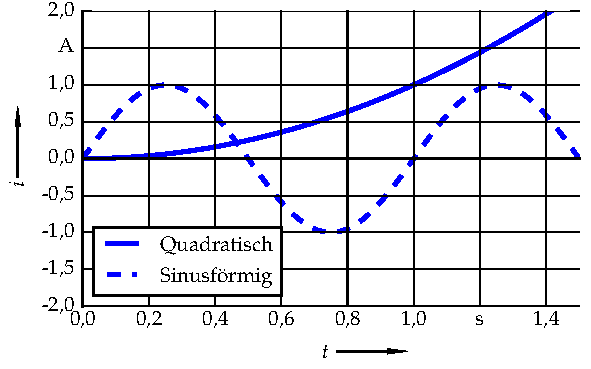
\includegraphics{figures/01plot/plotdin}\hfill{}\null

\caption{Dies ist eine Abbildung mit einer Abbildungsunterschrift, die die
Abbildung beschreibt.}
\label{fig:plots}

\end{figure}




\chapter{Tabellen}

Die Tabelle \ref{tab:komma} zeigt exemplarisch den Aufbau einer Tabelle.

\begin{longtable}[c]{|r|c|}
\caption{Messwertabelle verschiedener Unterstationen \label{tab:komma}}
\tabularnewline
\hline 
\textbf{Station} & \textbf{Messwert~(V)}\tabularnewline
\endfirsthead
\hline 
4711 & \hphantom{000}3,14\hphantom{0}\tabularnewline
\hline 
0815 & \phantom{000}2,74\hphantom{0}\tabularnewline
\hline 
0123456789 & \hphantom{000}2,345\tabularnewline
\hline 
0123456 & \hphantom{00}12,3\hphantom{00}\tabularnewline
\hline 
007 & 2345,3\hphantom{00}\tabularnewline
\hline 
\end{longtable}

Bei Tabellen sind insbesondere folgende Punkte wichtig:
\begin{itemize}
\item Zusammengehörige Zahlenwerte sind untereinander angeordnet, auch wenn
eine Anordnung nebeneinander Platzsparender ist. Untereinander angeordnete
Zahlenwerte sind leichter zu vergleichen.
\item Zahlenwerte sind untereinander am Komma ausgerichtet. Wenn die Zahl
kein Komma enthält, wird sie dort ausgerichtet, wo das Komma stehen
würde (Nach der letzten Ziffer).
\item Die Einheit steht entweder in der Spaltenüberschrift oder hinter jedem
Zahlenwert.
\item Die Tabellenüberschrift steht über der Tabelle, nicht unterhalb
\item Tabellen werden im Text erklärt.
\item Sehr große Tabellen mit Messwerten oder gerechneten Werten werden
häufig besser als Grafik dargestellt.
\end{itemize}




\chapter{Anhänge}

Für Anhänge gilt, dass das Dokument auch verständlich sein, soll,
wenn Anhänge fehlen würden. Lange Tabellen mit Messdaten können beispielsweise
in den Anhang aufgenommen werden, oder umfangreiche Konstruktionszeichnungen.
Als Beispiel sind hier in Anhang \ref{chap:Wichtige-Abbildung} und
Anhang \ref{chap:Wichtige-Tabelle} Anhänge beigefügt.

\chapter{Aufzählungen und Nummerierungen}

Insbesondere in den Naturwissenschaften ist es häufig sinnvoll statt
einem langen Fließtext eine Aufzählung oder eine Nummerierung zu verwenden.
Aufzählungen dienen:
\begin{itemize}
\item der Übersichtlichkeit
\item der Strukturierung
\item zur Nennung verschiedener Punkte, wenn keine Reihenfolge festgelegt
werden kann.
\end{itemize}
Eine Nummerierung wird verwendet, wenn eine Reihenfolge genannt werden
kann. Als Beispiel seien hier die fünf Sicherheitsregeln der Elektrotechnik
genannt:
\begin{enumerate}
\item Freischalten
\item Gegen Wiedereinschalten sichern
\item Spannungsfreiheit feststellen
\item Erden und Kurzschließen
\item Benachbarte unter Spannung stehende Teile abdecken oder abschranken.
\end{enumerate}

\chapter{Hyperlinks}

Hyperlinks können mit einem Rahmen umfasst werden, der am Display
angezeigt, aber nicht ausgedruckt wird. Dies zeigt die Abbildung \ref{fig:linkmitrahmen}.
Dies ist der Standardfall. Nicht alle PDF-Betrachtungsprogramme heben
hyperlinks optisch hervor. Das Programm SumatraPDF tut dies beispielsweise
nicht.

\begin{figure}
\hfill{}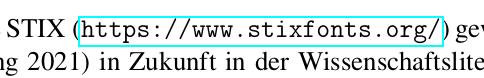
\includegraphics[width=5cm]{figures/05_rahmenumlinks/mitrahmen}\hfill{}\null

\caption{Hyperlink mit optischer Hervorhebung mit einem blauen Rahmen}
\label{fig:linkmitrahmen}
\end{figure}

Dies kann unterbunden werden mit folgenden Optionen des Paketes hyperref:

\bgroup\inputencoding{latin9}
\begin{lstlisting}
\usepackage[colorlinks=false,pdfborder={0 0 0}]  {hyperref}
\end{lstlisting}
\leavevmode\egroup

Die Abbildung \ref{fig:linkohnerahmen} zeigt das Ergebnis.

\begin{figure}
\hfill{}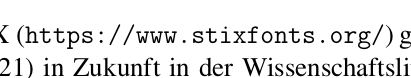
\includegraphics[width=5cm]{figures/05_rahmenumlinks/ohnerahmen}\hfill{}\null

\caption{Hyperlink ohe optischer Hervorhebung mit einem blauen Rahmen}
\label{fig:linkohnerahmen}
\end{figure}


\chapter{Quellcode}

In LaTeX gibt es das Paket Listings, mit dem recht komfortabel Quellcode
in das Dokument aufgenommen werden kann. Hier ist ein Beispiel: 

\lstinputlisting[caption={{Kurzer Batch-Code}},label={kurzerbatchcode}]{figures/02programmlisting/SplitPDFInSinglePages.ps}

Im folgenden Beispiel ist der Code farblich gekennzeichnet.

\lstinputlisting[language=Matlab,caption={Testunterschrift},label={foo}]{figures/04MatlabCode/matlabcode.m}

Hier ist ein weiteres Beispiel, welches einen Seitenumbruch, Listing-Unterschrift
und einen Querverweis (Es handelt sich um das Listing \ref{lstsehrlangeslisting})
auf das Listing enthält:

\lstinputlisting[captionpos=b,label={lstsehrlangeslisting},caption={Unterschrift des sehr langen Quellcodes}]{figures/02programmlisting/SehrLangerQuellCode.txt}

Hier ist ein Listing in einer Zeile \lstinline[language=C]|for(int i = 0, i<5,i++){i--;}print('a');struct A;// Kommentar|

Das ist ein inline-Code ohne Farben:  \lstinline[]|for(int i = 0, i<5,i++){i--;}print('a');struct A;// Kommentar|

\chapter{Zusammenfassung}

Hier wird beschrieben, welche Erkenntnisse sich aus der Arbeit ergeben.
Weiterhin kann hier auch angegeben werden, welche Themen weiter untersucht
werden können oder sollten.


\chapter{Hinweise zum Literaturverzeichnis}

Mit LaTeX/LyX kann ein Literaturverzeichnis mit oder ohne das System
Biblatex verwendet werden. Biblatex ließt eine Literaturdatenbank
ein und stellt ausgewählte Einträge im Literaturverzeichnis dar. In
dieser Variante der Vorlage wird gezeigt, wie ohne eine Literaturdatenbank
gearbeitet wird. Dabei ist die Literaturliste Teil des Hauptdokumentes.

Hier wird exemplarisch auf Literaturverweise eingegangen. Ein guter
Start in das Thema ,,Wissenschaftliches Schreiben`` ist in \cite{kuehtz}
gegeben.  Beim Zitieren von Internetquellen ist wichtig, permanente
Links zu verwenden. Beispielsweise wird in \cite{wikipediaelektrotechnik}
auf den Wikipedia-Artikel zur Elektrotechnik verwiesen. Hier ist ein
Zitat des Handbuches über das SI-System \cite{sisystemohnebiblatex},
einer Literatur, die im Internet zugänglich ist.
\begin{thebibliography}{1}
\bibitem{kuehtz}Kühtz, S. \textit{Wissenschaftlich formulieren.}
Paderborn: Schöningh, 2011

\bibitem{wikipediaelektrotechnik}Wikipedia-Autoren, siehe Versionsgeschichte..
\textit{Elektrotechnik -- Wikipedia, die freie Enzyklopädie }\textit{\emph{{[}Online{]}}}\textit{.}
2020-03-15 {[}Zugriff am 2021-03-16{]}. Verfügbar unter \url{https://de.wikipedia.org/w/index.php?title=Elektrotechnik&oldid=209822071}

\bibitem{sisystemohnebiblatex}International Bureau of Weights und
Measures (BIPM). The International System of Units (SI) {[}online{]}.
9th edition, 2019. {[}Zugrifff am 11. Nov. 2029{]}. Verfügbar unter:
\url{https: //www.bipm.org/documents/20126/41483022/SI-Brochure-9.pdf/fcf090b2-04e6- 88cc- 1149- c3e029ad8232?version=4.0&t=1736179646242&download=true.}

\end{thebibliography}

\appendix

\appendix

\chapter{Wichtige Abbildung}

\label{chap:Wichtige-Abbildung}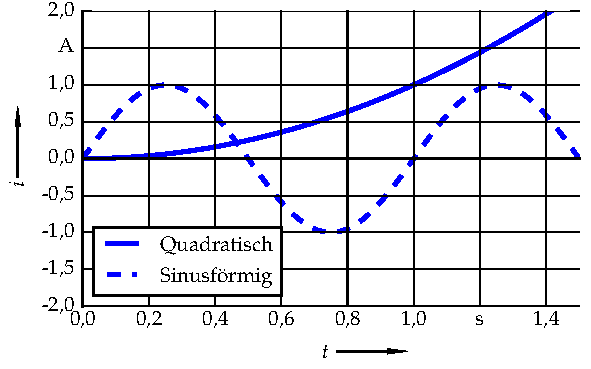
\includegraphics[width=10cm]{figures/01plot/plotdin}

\chapter{Wichtige Tabelle}

\label{chap:Wichtige-Tabelle}%
\begin{longtable}[c]{|r|c|}
\caption{Tabelle im Anhang \label{tab:wichtigetabelle}}
\tabularnewline
\hline 
\textbf{Station} & \textbf{Messwert~(V)}\tabularnewline
\endfirsthead
\hline 
4711 & \hphantom{000}3,14\hphantom{0}\tabularnewline
\hline 
0815 & \phantom{000}2,74\hphantom{0}\tabularnewline
\hline 
0123456789 & \hphantom{000}2,345\tabularnewline
\hline 
0123456 & \hphantom{00}12,3\hphantom{00}\tabularnewline
\hline 
007 & 2345,3\hphantom{00}\tabularnewline
\hline 
\end{longtable}

\end{document}
